\documentclass{article}
\usepackage[utf8]{inputenc}
\usepackage{tabularx} % extra features for tabular environment
\usepackage{amsmath}  % improve math presentation
\usepackage{graphicx} % takes care of graphic including machinery
\usepackage{xspace}
\usepackage{tikz}
\usepackage{enumitem}
\usetikzlibrary{babel}
\usepackage[american]{circuitikz}
\usetikzlibrary{calc}
\usepackage{siunitx}
\usepackage{pgfplots}
\usepackage[skins,theorems]{tcolorbox}
\tcbset{highlight math style={enhanced,
  colframe=red,colback=white,arc=0pt,boxrule=1pt}}
\pgfplotsset{width=10cm,compat=1.9}
\usepackage[margin=1in,letterpaper]{geometry} % decreases margins
\usepackage{cite} % takes care of citations
\usepackage[final]{hyperref} % adds hyper links inside the generated PDF file
\hypersetup{
colorlinks=true,       % false: boxed links; true: colored links
linkcolor=blue,        % color of internal links
citecolor=blue,        % color of links to bibliography
filecolor=magenta,     % color of file links
urlcolor=blue        
}
\usepackage{karnaugh-map}
%\usetikzlibrary{arrows, shapes.gates.logic.US, calc}
\usetikzlibrary{arrows,shapes.gates.logic.US,shapes.gates.logic.IEC,calc}

\begin{document}

\title{{\textbf{FPGA LAB ASSIGNMENT 1}}}
\author{\textbf{TADIPATRI UDAY KIRAN REDDY}\\\textbf{EE19BTECH11038}}
\maketitle

\section*{\hfil Problem \hfil}
Obtain the minimal form for the following Boolean expression using Karnaugh's Map.
\begin{equation*}
H (P, Q, R, S) = \sum (0, 1, 2, 3, 5, 7, 8, 9, 10, 14, 15)
\end{equation*}
\section*{\hfil Solution \hfill}
After simplification of the above truth table with Karnaugh's map shown in Figure \ref{fig:kmap_Av1}, we get the following boolean expression

\begin{equation*}
\label{eq:kmap_A}
H = Q^{\prime}S^{\prime} + Q^{\prime}R^{\prime} + P^{\prime}S + PQR 
\end{equation*}
We see that min terms are reduced from 11 to 4!. And corresponding NAND implementation is shown in Figure \ref{fig:nand}.

\begin{figure}[!h]
\resizebox {0.5\columnwidth} {!} {
\begin{karnaugh-map}[4][4][1][][]
    \maxterms{4,6,11,12,13}
    \minterms{0,1,2,3,5,7,8,9,10,14,15}
    \implicantedge{0}{1}{8}{9}
    \implicantedge{5}{7}{1}{3}
    \implicant{15}{14}
    \implicantcorner
    % note: posistion for start of \draw is (0, Y) where Y is
    % the Y size(number of cells high) in this case Y=2
    \draw[color=black, ultra thin] (0, 4) --
    node [pos=0.7, above right, anchor=south west] {$RS$} % Y label
    node [pos=0.7, below left, anchor=north east] {$PQ$} % X label
    ++(135:1);
        
\end{karnaugh-map}
}
\caption{K-Map for $H$.}
\label{fig:kmap_Av1}
\end{figure}
\newpage
\begin{figure}[!h]
\resizebox {1.12\columnwidth} {!} {



\def \globalscale {1.000000}
\begin{tikzpicture}[y=0.80pt, x=0.80pt, yscale=-\globalscale, xscale=\globalscale, inner sep=0pt, outer sep=0pt]
\begin{scope}[shift={(0,-402.41665)}]
  \begin{scope}[shift={(-1800.0135,-255)}]
    \path[xscale=0.982,yscale=1.019,fill=black,line join=miter,line cap=butt,line
      width=0.905pt] (1829.9742,831.0448) node[above right] (text1524) {P};



    \path[xscale=0.982,yscale=1.019,fill=black,line join=miter,line cap=butt,line
      width=0.905pt] (1831.2866,877.3930) node[above right] (text1524-3-7) {Q};



    \path[xscale=0.982,yscale=1.019,fill=black,line join=miter,line cap=butt,line
      width=0.905pt] (1831.0479,930.5998) node[above right] (text1524-3-9) {R};



    \path[xscale=0.982,yscale=1.019,fill=black,line join=miter,line cap=butt,line
      width=0.905pt] (1833.1068,976.3265) node[above right] (text1524-3-7-2) {S};



    \path[xscale=1.159,yscale=0.863,fill=black,line join=miter,line cap=butt,line
      width=1.364pt] (3075.1814,1243.6998) node[above right] (text1524-3-7-2-5) {H};



  \end{scope}
  \begin{scope}[cm={{1.83854,0.0,0.0,2.7678,(90.02885,362.29504)}}]
    \path[color=black,draw=black,line join=miter,line cap=round,miter
      limit=4.00,line width=2.835pt] (105.0000,24.4167) -- (105.0000,52.4166) --
      (119.0000,52.4166) .. controls (140.0000,52.4166) and (140.0000,24.4167) ..
      (119.0000,24.4167) -- cycle;



    \path[color=black,draw=black,line join=miter,line cap=round,miter
      limit=4.00,line width=1.890pt] (143.4134,38.4170) -- (154.0000,38.4166);



    \path[color=black,draw=black,line join=miter,line cap=round,miter
      limit=4.00,line width=1.890pt] (91.0000,31.4167) -- (105.0000,31.4167);



    \path[color=black,draw=black,line join=miter,line cap=round,miter
      limit=4.00,line width=1.890pt] (91.0000,45.4166) -- (105.0000,45.4166);



    \path[draw=black,line join=miter,line cap=round,miter limit=4.00,nonzero
      rule,line width=2.800pt] (138.2500,38.4166) circle (0.0988cm);



  \end{scope}
  \path[draw=black,line join=round,line cap=round,miter limit=4.00,nonzero
    rule,line width=4.263pt] (181.9872,449.2500) -- (257.3359,449.2500);



  \path[draw=black,line join=round,line cap=round,miter limit=4.00,nonzero
    rule,line width=4.263pt] (208.9753,487.9992) -- (257.3359,487.9992);



  \path[draw=black,line join=round,line cap=round,miter limit=4.00,nonzero
    rule,line width=4.263pt] (207.2125,487.9992) -- (207.2125,498.7426) --
    (207.2125,514.5856) -- (207.2125,524.1191) -- (207.2125,543.7822) --
    (207.2125,631.7410);



  \begin{scope}[cm={{1.23187,0.0,0.0,1.60415,(-28.01881,-236.66891)}}]
    \path[draw=black,line join=miter,line cap=round,miter limit=4.00,line
      width=3.032pt] (70.0000,514.4167) -- (54.2500,514.4167);



    \path[draw=black,line join=round,line cap=round,miter limit=4.00,nonzero
      rule,line width=3.032pt] (49.0000,514.4166) circle (0.1482cm);



    \path[draw=black,line join=miter,line cap=round,miter limit=4.00,line
      width=3.032pt] (70.0003,543.8455) -- (54.2503,543.8455);



    \path[draw=black,line join=round,line cap=round,miter limit=4.00,nonzero
      rule,line width=3.032pt] (49.0003,543.8455) circle (0.1482cm);



    \path[draw=black,line join=miter,line cap=round,miter limit=4.00,line
      width=3.032pt] (70.0003,577.6296) -- (54.2503,577.6296);



    \path[draw=black,line join=round,line cap=round,miter limit=4.00,nonzero
      rule,line width=3.032pt] (49.0003,577.6296) circle (0.1482cm);



    \path[draw=black,line join=miter,line cap=round,miter limit=4.00,line
      width=3.032pt] (70.0006,607.0585) -- (54.2506,607.0585);



    \path[draw=black,line join=round,line cap=round,miter limit=4.00,nonzero
      rule,line width=3.032pt] (49.0006,607.0584) circle (0.1482cm);



    \path[draw=black,line join=miter,line cap=round,miter limit=4.00,line
      width=3.032pt] (1414.6462,653.5725) -- (1430.3962,653.5725);



    \path[xscale=-1.000,yscale=1.000,draw=black,line join=round,line cap=round,miter
      limit=4.00,nonzero rule,line width=3.032pt] (-1435.6461,653.5724) circle
      (0.1482cm);



  \end{scope}
  \path[draw=black,line join=round,line cap=round,miter limit=4.00,nonzero
    rule,line width=4.263pt] (180.2243,451.0191) -- (180.2243,461.2718) --
    (180.2243,476.3909) -- (180.2243,485.4889) -- (180.2243,504.2536) --
    (180.2243,588.1940);



  \path[draw=black,line join=round,line cap=round,miter limit=4.00,nonzero
    rule,line width=4.263pt] (58.1886,588.5327) -- (67.3013,588.5327) --
    (80.7393,588.5327) -- (88.8258,588.5327) -- (105.5041,588.5327) --
    (180.1114,588.5327);



  \path[draw=black,line join=round,line cap=round,miter limit=4.00,nonzero
    rule,line width=4.263pt] (58.6916,635.7410) -- (69.8964,635.7410) --
    (86.4195,635.7410) -- (96.3625,635.7410) -- (116.8698,635.7410) --
    (208.6053,635.7410);



  \path[draw=black,line join=round,line cap=round,miter limit=4.00,nonzero
    rule,line width=4.263pt] (372.7213,468.6246) -- (391.5713,468.6246) --
    (419.3686,468.6246) -- (436.0958,468.6246) -- (470.5956,468.6246) --
    (624.9243,468.6246);



  \path[draw=black,line join=round,line cap=round,miter limit=4.00,nonzero
    rule,line width=4.985pt] (624.9243,449.2497) -- (628.4993,449.2497) --
    (633.7712,449.2497) -- (636.9436,449.2497) -- (643.4866,449.2497) --
    (672.7557,449.2497);



  \path[draw=black,line join=round,line cap=round,miter limit=4.00,nonzero
    rule,line width=4.263pt] (624.9243,487.9989) -- (628.4993,487.9989) --
    (633.7712,487.9989) -- (636.9436,487.9989) -- (643.4866,487.9989) --
    (672.7557,487.9989);



  \path[draw=black,line join=round,line cap=round,miter limit=4.00,nonzero
    rule,line width=4.263pt] (624.9243,449.2497) -- (624.9243,452.1459) --
    (624.9243,456.4167) -- (624.9243,458.9867) -- (624.9243,464.2874) --
    (624.9243,487.9989);



  \begin{scope}[cm={{1.83854,0.0,0.0,2.7678,(505.44868,362.29478)}}]
    \path[color=black,draw=black,line join=miter,line cap=round,miter
      limit=4.00,line width=2.835pt] (105.0000,24.4167) -- (105.0000,52.4166) --
      (119.0000,52.4166) .. controls (140.0000,52.4166) and (140.0000,24.4167) ..
      (119.0000,24.4167) -- cycle;



    \path[color=black,draw=black,line join=miter,line cap=round,miter
      limit=4.00,line width=1.890pt] (143.4134,38.4170) -- (154.0000,38.4166);



    \path[color=black,draw=black,line join=miter,line cap=round,miter
      limit=4.00,line width=1.890pt] (91.0000,31.4167) -- (105.0000,31.4167);



    \path[color=black,draw=black,line join=miter,line cap=round,miter
      limit=4.00,line width=1.890pt] (91.0000,45.4166) -- (105.0000,45.4166);



    \path[draw=black,line join=miter,line cap=round,miter limit=4.00,nonzero
      rule,line width=2.800pt] (138.2500,38.4166) circle (0.0988cm);



  \end{scope}
  \begin{scope}[cm={{1.83854,0.0,0.0,2.7678,(703.44162,451.20732)}}]
    \path[color=black,draw=black,line join=miter,line cap=round,miter
      limit=4.00,line width=2.835pt] (105.0000,24.4167) -- (105.0000,52.4166) --
      (119.0000,52.4166) .. controls (140.0000,52.4166) and (140.0000,24.4167) ..
      (119.0000,24.4167) -- cycle;



    \path[color=black,draw=black,line join=miter,line cap=round,miter
      limit=4.00,line width=1.890pt] (143.4134,38.4170) -- (154.0000,38.4166);



    \path[color=black,draw=black,line join=miter,line cap=round,miter
      limit=4.00,line width=1.890pt] (91.0000,31.4167) -- (105.0000,31.4167);



    \path[color=black,draw=black,line join=miter,line cap=round,miter
      limit=4.00,line width=1.890pt] (91.0000,45.4166) -- (105.0000,45.4166);



    \path[draw=black,line join=miter,line cap=round,miter limit=4.00,nonzero
      rule,line width=2.800pt] (138.2500,38.4166) circle (0.0988cm);



  \end{scope}
  \path[draw=black,line join=round,line cap=round,miter limit=4.00,nonzero
    rule,line width=4.263pt] (337.1288,576.9115) -- (377.0122,576.9115) --
    (435.8266,576.9115) -- (471.2186,576.9115) -- (544.2147,576.9115) --
    (870.7486,576.9115);



  \path[draw=black,line join=round,line cap=round,miter limit=4.00,nonzero
    rule,line width=4.263pt] (337.1288,575.2701) -- (337.1288,583.7060) --
    (337.1288,596.1460) -- (337.1288,603.6318) -- (337.1288,619.0715) --
    (337.1288,688.1376);



  \path[draw=black,line join=round,line cap=round,miter limit=4.00,nonzero
    rule,line width=4.263pt] (466.3777,673.7651) -- (469.9527,673.7651) --
    (475.2246,673.7651) -- (478.3970,673.7651) -- (484.9400,673.7651) --
    (514.2091,673.7651);



  \path[draw=black,line join=round,line cap=round,miter limit=4.00,nonzero
    rule,line width=4.263pt] (466.3777,712.5143) -- (469.9527,712.5143) --
    (475.2246,712.5143) -- (478.3970,712.5143) -- (484.9400,712.5143) --
    (514.2091,712.5143);



  \path[draw=black,line join=round,line cap=round,miter limit=4.00,nonzero
    rule,line width=4.245pt] (466.3777,673.7651) -- (466.3777,676.6613) --
    (466.3777,680.9321) -- (466.3777,683.5021) -- (466.3777,688.8028) --
    (466.3777,712.5143);



  \begin{scope}[cm={{1.83854,0.0,0.0,2.7678,(346.90209,586.81013)}}]
    \path[color=black,draw=black,line join=miter,line cap=round,miter
      limit=4.00,line width=2.835pt] (105.0000,24.4167) -- (105.0000,52.4166) --
      (119.0000,52.4166) .. controls (140.0000,52.4166) and (140.0000,24.4167) ..
      (119.0000,24.4167) -- cycle;



    \path[color=black,draw=black,line join=miter,line cap=round,miter
      limit=4.00,line width=1.890pt] (143.4134,38.4170) -- (154.0000,38.4166);



    \path[color=black,draw=black,line join=miter,line cap=round,miter
      limit=4.00,line width=1.890pt] (91.0000,31.4167) -- (105.0000,31.4167);



    \path[color=black,draw=black,line join=miter,line cap=round,miter
      limit=4.00,line width=1.890pt] (91.0000,45.4166) -- (105.0000,45.4166);



    \path[draw=black,line join=miter,line cap=round,miter limit=4.00,nonzero
      rule,line width=2.800pt] (138.2500,38.4166) circle (0.0988cm);



  \end{scope}
  \path[draw=black,line join=round,line cap=round,miter limit=4.00,nonzero
    rule,line width=4.263pt] (784.6196,468.6243) -- (787.4133,468.6243) --
    (791.5330,468.6243) -- (794.0122,468.6243) -- (799.1253,468.6243) --
    (821.9979,468.6243);



  \path[draw=black,line join=round,line cap=round,miter limit=4.00,nonzero
    rule,line width=4.263pt] (822.4250,470.4696) -- (822.4250,475.3581) --
    (822.4250,482.5669) -- (822.4250,486.9049) -- (822.4250,495.8520) --
    (822.4250,535.8749);



  \path[draw=black,line join=round,line cap=round,miter limit=4.00,nonzero
    rule,line width=4.263pt] (870.9731,538.1623) -- (867.3102,538.1623) --
    (861.9087,538.1623) -- (858.6583,538.1623) -- (851.9543,538.1623) --
    (821.9656,538.1623);



  \path[draw=black,line join=round,line cap=round,miter limit=4.00,nonzero
    rule,line width=4.263pt] (208.6359,635.7410) -- (220.7939,635.7410) --
    (238.7228,635.7410) -- (249.5117,635.7410) -- (271.7637,635.7410) --
    (371.3038,635.7410);



  \path[draw=black,line join=round,line cap=round,miter limit=4.00,nonzero
    rule,line width=4.263pt] (371.8230,635.6829) -- (371.8230,639.6532) --
    (371.8230,645.5079) -- (371.8230,649.0311) -- (371.8230,656.2975) --
    (371.8230,688.8028);



  \path[draw=black,line join=round,line cap=round,miter limit=4.00,nonzero
    rule,line width=4.263pt] (464.4823,688.8028) -- (457.5568,688.8028) --
    (447.3441,688.8028) -- (441.1986,688.8028) -- (428.5233,688.8028) --
    (371.8230,688.8028);



  \path[draw=black,line join=round,line cap=round,miter limit=4.00,nonzero
    rule,line width=4.263pt] (58.2121,689.9358) -- (78.8582,689.9358) --
    (109.3040,689.9358) -- (127.6250,689.9358) -- (165.4121,689.9358) --
    (334.4454,689.9358);



  \path[draw=black,line join=round,line cap=round,miter limit=4.00,nonzero
    rule,line width=4.263pt] (986.5766,538.3643) -- (990.1516,538.3643) --
    (995.4234,538.3643) -- (998.5958,538.3643) -- (1005.1389,538.3643) --
    (1034.4079,538.3643);



  \path[draw=black,line join=round,line cap=round,miter limit=4.00,nonzero
    rule,line width=4.263pt] (986.5766,577.1135) -- (990.1516,577.1135) --
    (995.4234,577.1135) -- (998.5958,577.1135) -- (1005.1389,577.1135) --
    (1034.4079,577.1135);



  \path[draw=black,line join=round,line cap=round,miter limit=4.00,nonzero
    rule,line width=4.245pt] (986.5766,538.3643) -- (986.5766,541.2605) --
    (986.5766,545.5313) -- (986.5766,548.1013) -- (986.5766,553.4020) --
    (986.5766,577.1135);



  \begin{scope}[cm={{1.83854,0.0,0.0,2.7678,(867.10089,451.40935)}}]
    \path[color=black,draw=black,line join=miter,line cap=round,miter
      limit=4.00,line width=2.835pt] (105.0000,24.4167) -- (105.0000,52.4166) --
      (119.0000,52.4166) .. controls (140.0000,52.4166) and (140.0000,24.4167) ..
      (119.0000,24.4167) -- cycle;



    \path[color=black,draw=black,line join=miter,line cap=round,miter
      limit=4.00,line width=1.890pt] (143.4134,38.4170) -- (154.0000,38.4166);



    \path[color=black,draw=black,line join=miter,line cap=round,miter
      limit=4.00,line width=1.890pt] (91.0000,31.4167) -- (105.0000,31.4167);



    \path[color=black,draw=black,line join=miter,line cap=round,miter
      limit=4.00,line width=1.890pt] (91.0000,45.4166) -- (105.0000,45.4166);



    \path[draw=black,line join=miter,line cap=round,miter limit=4.00,nonzero
      rule,line width=2.800pt] (138.2500,38.4166) circle (0.0988cm);



  \end{scope}
  \begin{scope}[cm={{1.83854,0.0,0.0,2.7678,(346.8739,721.07238)}}]
    \path[color=black,draw=black,line join=miter,line cap=round,miter
      limit=4.00,line width=2.835pt] (105.0000,24.4167) -- (105.0000,52.4166) --
      (119.0000,52.4166) .. controls (140.0000,52.4166) and (140.0000,24.4167) ..
      (119.0000,24.4167) -- cycle;



    \path[color=black,draw=black,line join=miter,line cap=round,miter
      limit=4.00,line width=1.890pt] (143.4134,38.4170) -- (154.0000,38.4166);



    \path[color=black,draw=black,line join=miter,line cap=round,miter
      limit=4.00,line width=1.890pt] (91.0000,31.4167) -- (105.0000,31.4167);



    \path[color=black,draw=black,line join=miter,line cap=round,miter
      limit=4.00,line width=1.890pt] (91.0000,45.4166) -- (105.0000,45.4166);



    \path[draw=black,line join=miter,line cap=round,miter limit=4.00,nonzero
      rule,line width=2.800pt] (138.2500,38.4166) circle (0.0988cm);



  \end{scope}
  \path[draw=black,line join=round,line cap=round,miter limit=4.00,nonzero
    rule,line width=4.263pt] (292.9217,689.9358) -- (292.9217,698.7622) --
    (292.9217,711.7779) -- (292.9217,719.6103) -- (292.9217,735.7645) --
    (292.9217,808.0273);



  \path[draw=black,line join=round,line cap=round,miter limit=4.00,nonzero
    rule,line width=4.263pt] (514.1809,808.0273) -- (497.6437,808.0273) --
    (473.2570,808.0273) -- (458.5822,808.0273) -- (428.3152,808.0273) --
    (292.9217,808.0273);



  \path[draw=black,line join=round,line cap=round,miter limit=4.00,nonzero
    rule,line width=4.263pt] (236.8487,737.1441) -- (223.4290,737.1441) --
    (203.6397,737.1441) -- (191.7313,737.1441) -- (167.1703,737.1441) --
    (57.3011,737.1441);



  \path[draw=black,line join=round,line cap=round,miter limit=4.00,nonzero
    rule,line width=4.263pt] (236.8487,846.8674) -- (236.8487,838.7852) --
    (236.8487,826.8667) -- (236.8487,819.6947) -- (236.8487,804.9023) --
    (236.8487,738.7316);



  \path[draw=black,line join=round,line cap=round,miter limit=4.00,nonzero
    rule,line width=4.263pt] (236.8487,846.7765) -- (257.5768,846.7765) --
    (288.1438,846.7765) -- (306.5377,846.7765) -- (344.4751,846.7765) --
    (514.1809,846.7765);



  \path[draw=black,line join=round,line cap=round,miter limit=4.00,nonzero
    rule,line width=4.985pt] (171.5109,900.4136) -- (175.0859,900.4136) --
    (180.3578,900.4136) -- (183.5301,900.4136) -- (190.0732,900.4136) --
    (219.3423,900.4136);



  \path[draw=black,line join=round,line cap=round,miter limit=4.00,nonzero
    rule,line width=4.985pt] (171.5109,939.1627) -- (175.0859,939.1627) --
    (180.3578,939.1627) -- (183.5301,939.1627) -- (190.0732,939.1627) --
    (219.3423,939.1627);



  \path[draw=black,line join=round,line cap=round,miter limit=4.00,nonzero
    rule,line width=4.245pt] (171.5109,900.4136) -- (171.5109,903.3097) --
    (171.5109,907.5806) -- (171.5109,910.1506) -- (171.5109,915.4513) --
    (171.5109,939.1627);



  \begin{scope}[cm={{1.83854,0.0,0.0,2.7678,(52.03527,813.4586)}}]
    \path[color=black,draw=black,line join=miter,line cap=round,miter
      limit=4.00,line width=2.835pt] (105.0000,24.4167) -- (105.0000,52.4166) --
      (119.0000,52.4166) .. controls (140.0000,52.4166) and (140.0000,24.4167) ..
      (119.0000,24.4167) -- cycle;



    \path[color=black,draw=black,line join=miter,line cap=round,miter
      limit=4.00,line width=1.890pt] (143.4134,38.4170) -- (154.0000,38.4166);



    \path[color=black,draw=black,line join=miter,line cap=round,miter
      limit=4.00,line width=1.890pt] (91.0000,31.4167) -- (105.0000,31.4167);



    \path[color=black,draw=black,line join=miter,line cap=round,miter
      limit=4.00,line width=1.890pt] (91.0000,45.4166) -- (105.0000,45.4166);



    \path[draw=black,line join=miter,line cap=round,miter limit=4.00,nonzero
      rule,line width=2.800pt] (138.2500,38.4166) circle (0.0988cm);



  \end{scope}
  \path[draw=black,line join=round,line cap=round,miter limit=4.00,nonzero
    rule,line width=4.263pt] (111.1827,917.6659) -- (111.1827,904.2994) --
    (111.1827,884.5884) -- (111.1827,872.7271) -- (111.1827,848.2633) --
    (111.1827,738.8291);



  \path[draw=black,line join=round,line cap=round,miter limit=4.00,nonzero
    rule,line width=4.257pt] (111.7935,919.5861) -- (116.1860,919.5861) --
    (122.6634,919.5861) -- (126.5612,919.5861) -- (134.6004,919.5861) --
    (170.5626,919.5861);



  \begin{scope}[cm={{1.83854,0.0,0.0,2.7678,(349.95878,879.8952)}}]
    \path[color=black,draw=black,line join=miter,line cap=round,miter
      limit=4.00,line width=2.835pt] (105.0000,24.4167) -- (105.0000,52.4166) --
      (119.0000,52.4166) .. controls (140.0000,52.4166) and (140.0000,24.4167) ..
      (119.0000,24.4167) -- cycle;



    \path[color=black,draw=black,line join=miter,line cap=round,miter
      limit=4.00,line width=1.890pt] (143.4134,38.4170) -- (154.0000,38.4166);



    \path[color=black,draw=black,line join=miter,line cap=round,miter
      limit=4.00,line width=1.890pt] (91.0000,31.4167) -- (105.0000,31.4167);



    \path[color=black,draw=black,line join=miter,line cap=round,miter
      limit=4.00,line width=1.890pt] (91.0000,45.4166) -- (105.0000,45.4166);



    \path[draw=black,line join=miter,line cap=round,miter limit=4.00,nonzero
      rule,line width=2.800pt] (138.2500,38.4166) circle (0.0988cm);



  \end{scope}
  \path[draw=black,line join=round,line cap=round,miter limit=4.00,nonzero
    rule,line width=4.263pt] (143.2336,1005.5993) -- (143.2336,974.4272) --
    (143.2336,928.4590) -- (143.2336,900.7974) -- (143.2336,843.7451) --
    (143.2336,588.5327);



  \path[draw=black,line join=round,line cap=round,miter limit=4.00,nonzero
    rule,line width=4.263pt] (143.2336,1005.5993) -- (171.1893,1005.5993) --
    (212.4143,1005.5993) -- (237.2217,1005.5993) -- (288.3871,1005.5993) --
    (517.2658,1005.5993);



  \path[draw=black,line join=round,line cap=round,miter limit=4.00,nonzero
    rule,line width=4.263pt] (331.5093,919.7882) -- (341.7276,919.7882) --
    (356.7962,919.7882) -- (365.8638,919.7882) -- (384.5658,919.7882) --
    (468.2256,919.7882);



  \path[draw=black,line join=round,line cap=round,miter limit=4.00,nonzero
    rule,line width=3.547pt] (468.4992,919.0851) -- (468.4992,922.6620) --
    (468.4992,927.9366) -- (468.4992,931.1106) -- (468.4992,937.6570) --
    (468.4992,966.9412);



  \path[draw=black,line join=round,line cap=round,miter limit=4.00,nonzero
    rule,line width=3.877pt] (468.4992,966.8502) -- (472.1441,966.8502) --
    (477.5191,966.8502) -- (480.7535,966.8502) -- (487.4244,966.8502) --
    (517.2658,966.8502);



  \begin{scope}[cm={{1.83854,0.0,0.0,2.7678,(605.02199,650.6779)}}]
    \path[color=black,draw=black,line join=miter,line cap=round,miter
      limit=4.00,line width=2.835pt] (105.0000,24.4167) -- (105.0000,52.4166) --
      (119.0000,52.4166) .. controls (140.0000,52.4166) and (140.0000,24.4167) ..
      (119.0000,24.4167) -- cycle;



    \path[color=black,draw=black,line join=miter,line cap=round,miter
      limit=4.00,line width=1.890pt] (143.4134,38.4170) -- (154.0000,38.4166);



    \path[color=black,draw=black,line join=miter,line cap=round,miter
      limit=4.00,line width=1.890pt] (91.0000,31.4167) -- (105.0000,31.4167);



    \path[color=black,draw=black,line join=miter,line cap=round,miter
      limit=4.00,line width=1.890pt] (91.0000,45.4166) -- (105.0000,45.4166);



    \path[draw=black,line join=miter,line cap=round,miter limit=4.00,nonzero
      rule,line width=2.800pt] (138.2500,38.4166) circle (0.0988cm);



  \end{scope}
  \path[draw=black,line join=round,line cap=round,miter limit=4.00,nonzero
    rule,line width=3.378pt] (730.5776,693.3711) -- (730.5776,696.6154) --
    (730.5776,701.3997) -- (730.5776,704.2786) -- (730.5776,710.2165) --
    (730.5776,736.7784);



  \path[draw=black,line join=round,line cap=round,miter limit=4.00,nonzero
    rule,line width=4.263pt] (730.5776,693.1397) -- (723.0628,693.1397) --
    (711.9811,693.1397) -- (705.3127,693.1397) -- (691.5589,693.1397) --
    (630.0342,693.1397);



  \path[draw=black,line join=round,line cap=round,miter limit=4.00,nonzero
    rule,line width=4.263pt] (771.8603,737.6329) -- (768.7328,737.6329) --
    (764.1207,737.6329) -- (761.3454,737.6329) -- (755.6212,737.6329) --
    (730.0153,737.6329);



  \path[draw=black,line join=round,line cap=round,miter limit=4.00,nonzero
    rule,line width=3.619pt] (730.9690,777.4872) -- (730.9690,781.2221) --
    (730.9690,786.7298) -- (730.9690,790.0441) -- (730.9690,796.8799) --
    (730.9690,827.4583);



  \path[draw=black,line join=round,line cap=round,miter limit=4.00,nonzero
    rule,line width=4.263pt] (630.8216,827.7248) -- (638.3068,827.7248) --
    (649.3448,827.7248) -- (655.9870,827.7248) -- (669.6866,827.7248) --
    (730.9690,827.7248);



  \path[draw=black,line join=round,line cap=round,miter limit=4.00,nonzero
    rule,line width=4.263pt] (730.4083,776.5035) -- (733.5273,776.5035) --
    (738.1268,776.5035) -- (740.8946,776.5035) -- (746.6031,776.5035) --
    (772.1394,776.5035);



  \begin{scope}[cm={{1.83854,0.0,0.0,2.7678,(1040.8051,569.07991)}}]
    \path[color=black,draw=black,line join=miter,line cap=round,miter
      limit=4.00,line width=2.835pt] (105.0000,24.4167) -- (105.0000,52.4166) --
      (119.0000,52.4166) .. controls (140.0000,52.4166) and (140.0000,24.4167) ..
      (119.0000,24.4167) -- cycle;



    \path[color=black,draw=black,line join=miter,line cap=round,miter
      limit=4.00,line width=1.890pt] (143.4134,38.4170) -- (154.0000,38.4166);



    \path[color=black,draw=black,line join=miter,line cap=round,miter
      limit=4.00,line width=1.890pt] (91.0000,31.4167) -- (105.0000,31.4167);



    \path[color=black,draw=black,line join=miter,line cap=round,miter
      limit=4.00,line width=1.890pt] (91.0000,45.4166) -- (105.0000,45.4166);



    \path[draw=black,line join=miter,line cap=round,miter limit=4.00,nonzero
      rule,line width=2.800pt] (138.2500,38.4166) circle (0.0988cm);



  \end{scope}
  \begin{scope}[cm={{1.83854,0.0,0.0,2.7678,(1266.0785,705.22805)}}]
    \path[color=black,draw=black,line join=miter,line cap=round,miter
      limit=4.00,line width=2.835pt] (105.0000,24.4167) -- (105.0000,52.4166) --
      (119.0000,52.4166) .. controls (140.0000,52.4166) and (140.0000,24.4167) ..
      (119.0000,24.4167) -- cycle;



    \path[color=black,draw=black,line join=miter,line cap=round,miter
      limit=4.00,line width=1.890pt] (143.4134,38.4170) -- (154.0000,38.4166);



    \path[color=black,draw=black,line join=miter,line cap=round,miter
      limit=4.00,line width=1.890pt] (91.0000,31.4167) -- (105.0000,31.4167);



    \path[color=black,draw=black,line join=miter,line cap=round,miter
      limit=4.00,line width=1.890pt] (91.0000,45.4166) -- (105.0000,45.4166);



    \path[draw=black,line join=miter,line cap=round,miter limit=4.00,nonzero
      rule,line width=2.800pt] (138.2500,38.4166) circle (0.0988cm);



  \end{scope}
  \path[draw=black,line join=round,line cap=round,miter limit=4.00,nonzero
    rule,line width=4.263pt] (1550.9763,792.3850) -- (1554.5513,792.3850) --
    (1559.8231,792.3850) -- (1562.9955,792.3850) -- (1569.5386,792.3850) --
    (1598.8077,792.3850);



  \path[draw=black,line join=round,line cap=round,miter limit=4.00,nonzero
    rule,line width=4.263pt] (1550.9763,831.1342) -- (1554.5513,831.1342) --
    (1559.8231,831.1342) -- (1562.9955,831.1342) -- (1569.5386,831.1342) --
    (1598.8077,831.1342);



  \path[draw=black,line join=round,line cap=round,miter limit=4.00,nonzero
    rule,line width=4.263pt] (1550.9763,792.3850) -- (1550.9763,795.2812) --
    (1550.9763,799.5521) -- (1550.9763,802.1220) -- (1550.9763,807.4227) --
    (1550.9763,831.1342);



  \begin{scope}[cm={{1.83854,0.0,0.0,2.7678,(1431.5006,705.43008)}}]
    \path[color=black,draw=black,line join=miter,line cap=round,miter
      limit=4.00,line width=2.835pt] (105.0000,24.4167) -- (105.0000,52.4166) --
      (119.0000,52.4166) .. controls (140.0000,52.4166) and (140.0000,24.4167) ..
      (119.0000,24.4167) -- cycle;



    \path[color=black,draw=black,line join=miter,line cap=round,miter
      limit=4.00,line width=1.890pt] (143.4134,38.4170) -- (154.0000,38.4166);



    \path[color=black,draw=black,line join=miter,line cap=round,miter
      limit=4.00,line width=1.890pt] (91.0000,31.4167) -- (105.0000,31.4167);



    \path[color=black,draw=black,line join=miter,line cap=round,miter
      limit=4.00,line width=1.890pt] (91.0000,45.4166) -- (105.0000,45.4166);



    \path[draw=black,line join=miter,line cap=round,miter limit=4.00,nonzero
      rule,line width=2.800pt] (138.2500,38.4166) circle (0.0988cm);



  \end{scope}
  \path[draw=black,line join=round,line cap=round,miter limit=4.00,nonzero
    rule,line width=4.258pt] (1146.2779,557.7389) -- (1150.6730,557.7389) --
    (1157.1543,557.7389) -- (1161.0546,557.7389) -- (1169.0987,557.7389) --
    (1205.0826,557.7389);



  \path[draw=black,line join=round,line cap=round,miter limit=4.00,nonzero
    rule,line width=5.054pt] (1206.8455,558.9342) -- (1206.8455,566.1966) --
    (1206.8455,576.9060) -- (1206.8455,583.3505) -- (1206.8455,596.6423) --
    (1206.8455,656.1005);



  \path[draw=black,line join=round,line cap=round,miter limit=4.00,nonzero
    rule,line width=4.263pt] (885.2624,757.0074) -- (909.2743,757.0074) --
    (944.6837,757.0074) -- (965.9915,757.0074) -- (1009.9392,757.0074) --
    (1206.5299,757.0074);



  \path[draw=black,line join=round,line cap=round,miter limit=4.00,nonzero
    rule,line width=4.263pt] (1208.1122,694.6348) -- (1208.1122,699.2582) --
    (1208.1122,706.0760) -- (1208.1122,710.1787) -- (1208.1122,718.6406) --
    (1208.1122,756.4929);



  \path[draw=black,line join=round,line cap=round,miter limit=4.00,nonzero
    rule,line width=4.263pt] (628.5818,986.2247) -- (683.5754,986.2247) --
    (764.6721,986.2247) -- (813.4727,986.2247) -- (914.1238,986.2247) --
    (1364.3679,986.2247);



  \path[draw=black,line join=round,line cap=round,miter limit=4.00,nonzero
    rule,line width=4.263pt] (1364.3679,831.5438) -- (1364.3679,843.1048) --
    (1364.3679,860.1534) -- (1364.3679,870.4126) -- (1364.3679,891.5720) --
    (1364.3679,986.2247);



  \path[draw=black,line join=round,line cap=round,miter limit=4.00,nonzero
    rule,line width=4.676pt] (1435.1125,830.9322) -- (1429.8114,830.9322) --
    (1421.9938,830.9322) -- (1417.2897,830.9322) -- (1407.5872,830.9322) --
    (1364.1850,830.9322);



  \path[draw=black,line join=round,line cap=round,miter limit=4.00,nonzero
    rule,line width=4.676pt] (1433.3855,792.1830) -- (1428.0844,792.1830) --
    (1420.2668,792.1830) -- (1415.5626,792.1830) -- (1405.8601,792.1830) --
    (1362.4580,792.1830);



  \path[draw=black,line join=round,line cap=round,miter limit=4.00,nonzero
    rule,line width=3.455pt] (1361.4180,675.4095) -- (1358.5239,675.4095) --
    (1354.2562,675.4095) -- (1351.6882,675.4095) -- (1346.3913,675.4095) --
    (1322.6971,675.4095);



  \path[draw=black,line join=round,line cap=round,miter limit=4.00,nonzero
    rule,line width=4.263pt] (1363.3823,676.4498) -- (1363.3823,685.0999) --
    (1363.3823,697.8557) -- (1363.3823,705.5317) -- (1363.3823,721.3633) --
    (1363.3823,792.1830);



\end{scope}

\end{tikzpicture}

}
\caption{NAND implementation of $H$.}
\label{fig:nand}
\end{figure}

\subsection*{Optimality verfication}
To verify the optimality of above result, The given min terms are given to \textit{Quine-McCluskey} algorithm implemented \href{https://github.com/TUdayKiranReddy/FPGA_Lab/tree/main/Assignments/Assignment_1/Quine_Mccluskey}{here}. This was implemented using \textit{cvxpy}.
\begin{figure}[!h]
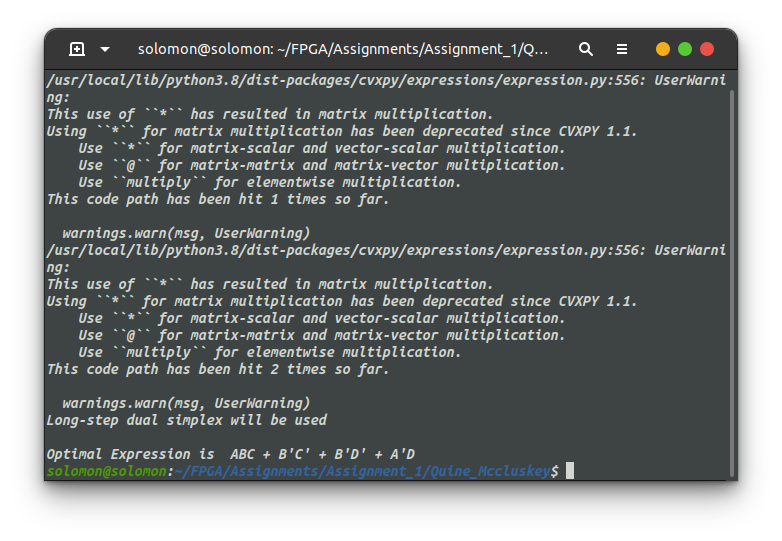
\includegraphics[scale=0.45]{./figs/opt.png}
\end{figure}

\textit{NOTE:- Here A, B, C, and D corresponds to P, Q, R, and S respectively.}
\newpage
\subsection*{Boolean expression verification}
A \href{https://github.com/TUdayKiranReddy/FPGA_Lab/tree/main/Assignments/Assignment_1/codes/verification_testbench.c}{testbench} was created using NAND logic to verify the correctness of the obtained boolean expression.
\begin{figure}[h!]
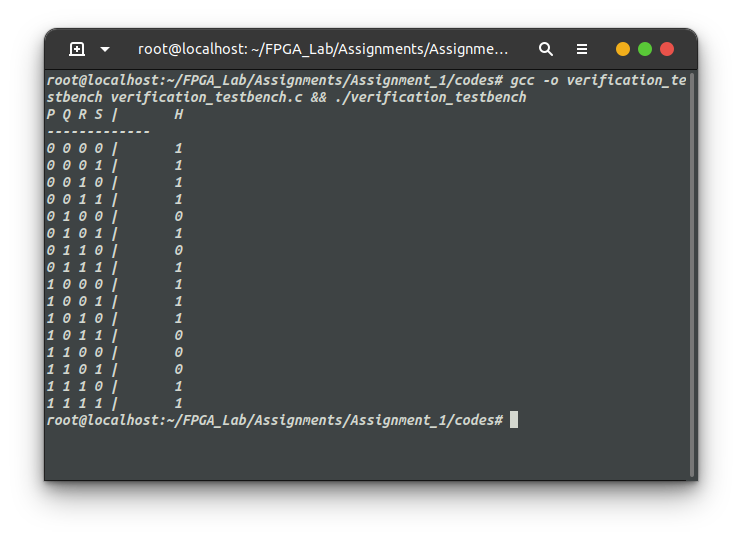
\includegraphics[scale=0.45]{./figs/ver.png}
\end{figure}
\end{document}